\documentclass[11pt]{article}

%%%%%%%%%%%%%%Include Packages%%%%%%%%%%%%%%%%%%%%%%%%%%
\usepackage{xcolor}
\usepackage{mathtools}
\usepackage[a4paper, total={6in, 8in}, margin=1.25in]{geometry}
\usepackage{amsmath}
\usepackage{amssymb}
\usepackage{paralist}
\usepackage{rsfso}
\usepackage{amsthm}
\usepackage{wasysym}
\usepackage[inline]{enumitem}   
\usepackage{hyperref}
\usepackage{tocloft}
\usepackage{titlesec}
\usepackage{colortbl}
%%%%%%%%%%%%%%%%%%%%%%%%%%%%%%%%%%%%%%%%%%%%%%%%%%%%%%%%



\begin{document}
\Large \noindent \textbf{Physics 5C Discussion (Week 2)}\\
\normalsize
Department of Physics and Astronomy, UCLA\\
%\noindent TA: Jinyan Miao (jnmiu@ucla.edu)\\
%Office hours: Thursday 10-11 AM $\&$ 1-2 PM at PAB 2-429\\
%Tutoring center hours: Friday 2-3 PM at PAB 2-429 (Zoom room also available)\\
\noindent\rule{8cm}{0.4pt}\\

\noindent\textbf{Problem 1}: There are two point charges $q_1$ and $q_2$ fixed in space. Now Jinyan throws a third point charge $q_3$ into the region, such that $q_3$ will have some initial velocity, as indicated in the figure. 
\begin{center}
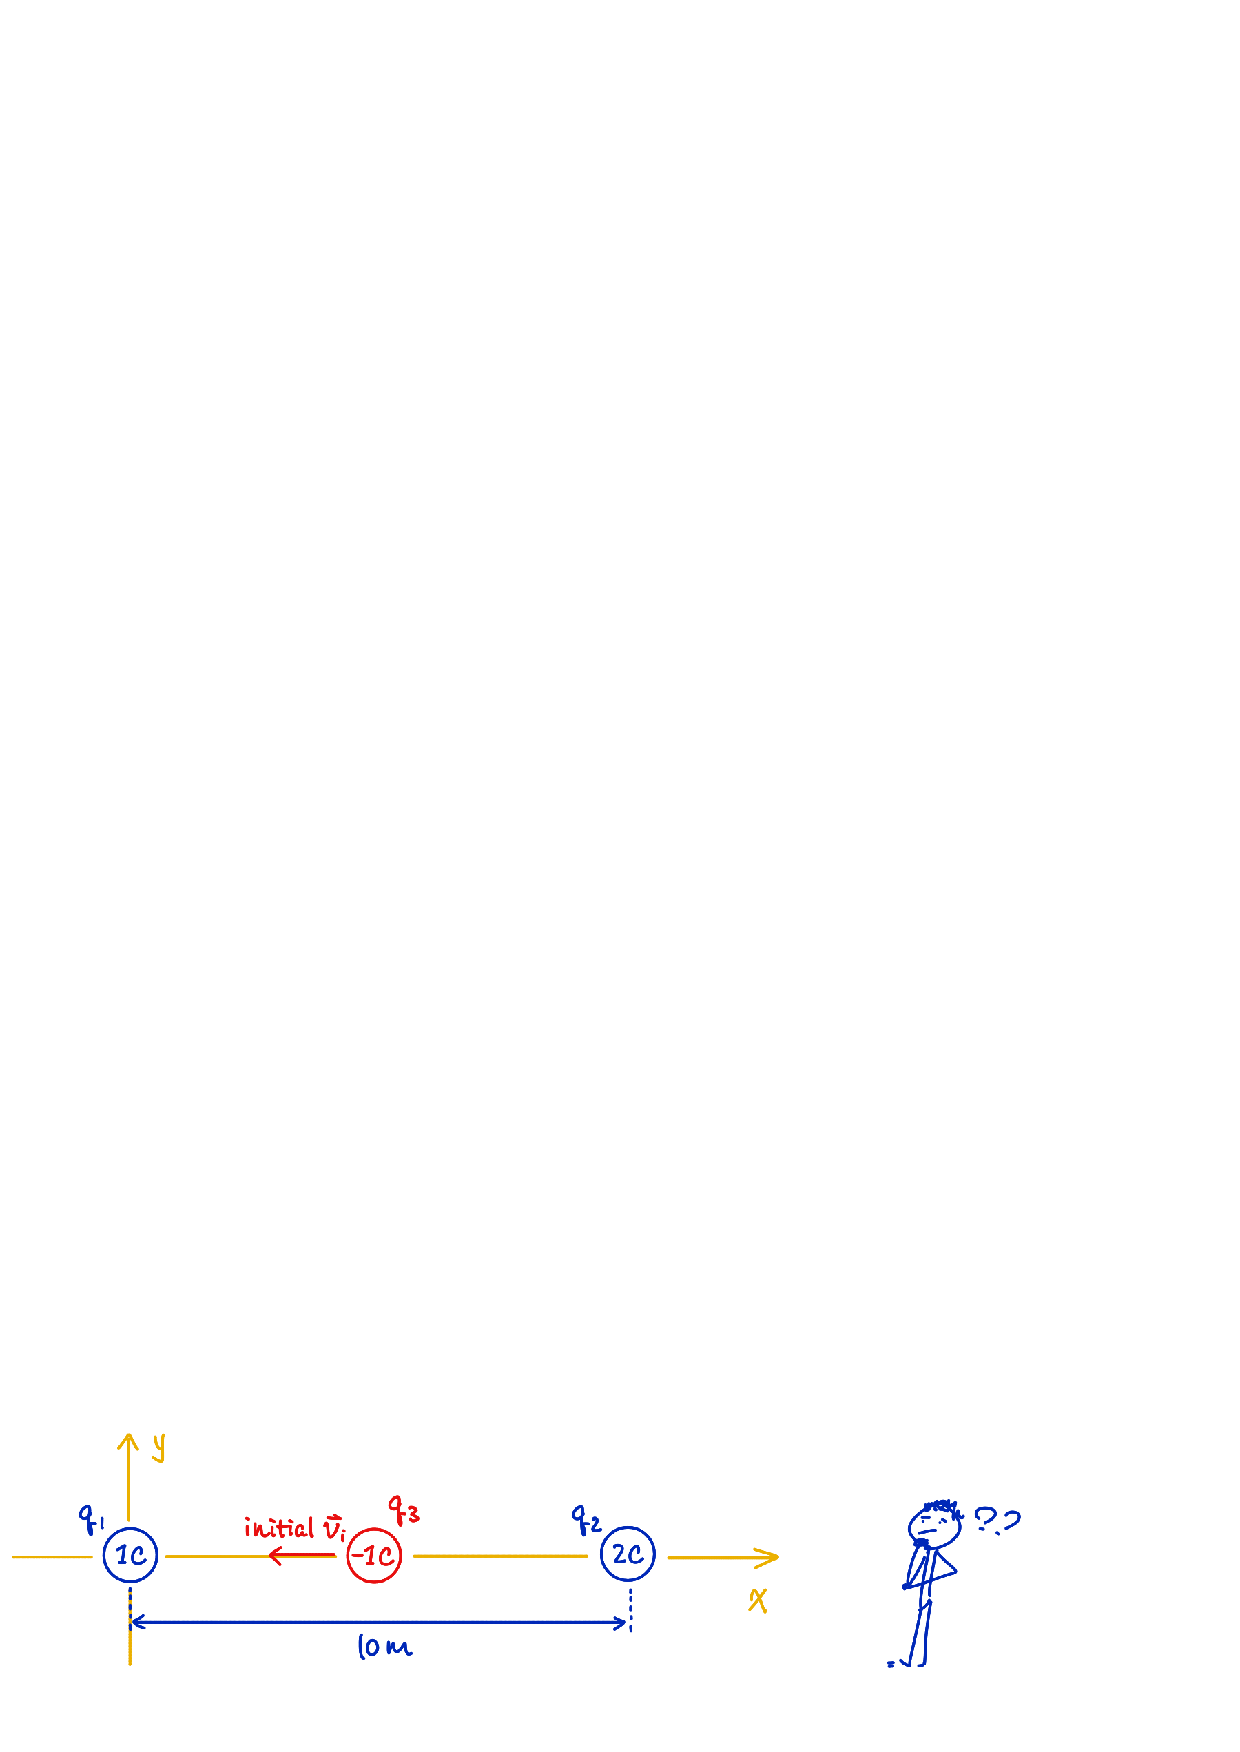
\includegraphics[scale=0.8]{chargeLine}
\end{center}
\noindent $q_1 = 1\,$C is fixed at $\vec{x}_1 = (0,0)$\,m. \\
$q_2=2\,$C is fixed at $\vec{x}_2 =(10,0)$\,m. \\
$q_3=-1$\,C is initially between $q_1$ and $q_2$ on the $x$-axis with some initial velocity.\\
The Coulomb constant $k = 8.99 \cdot 10^9$\,Nm$^2$/C$^2$.\\

\noindent\textbf{Part (a)} Sketch the electric field produced by the source charges $q_1$ and $q_2$.\\

\noindent\textbf{Part (b)} At which point in space does the test charge $q_3$ experience a zero net force (neglect gravity and friction, only consider the electric force)? \\

\noindent \textbf{Part (c)}
When $q_3$ is located at the point where it experiences zero net force, find the electric force experienced by $q_2$ in that configuration.\\

\noindent\textbf{Part (d)} Suppose $q_3$ is initially at $\vec{x}_3 = (5,0)$\,m, not the point where it experiences zero net force, with initial velocity $\vec{v}_i = (-1,0)$\,m/s. Qualitatively describe the motion of $q_3$ in such a configuration. How will it move under the electric forces from the source charges? Is there any way we can describe its motion quantitatively? \footnote{No need to do any calculation for this part, just describe in words.}\\



\newpage
\noindent\textbf{Problem 2}: [This problem is not too difficult, try to solve it when you get time.]\\ Now we change the configuration a little bit, see the figure.
\begin{center}
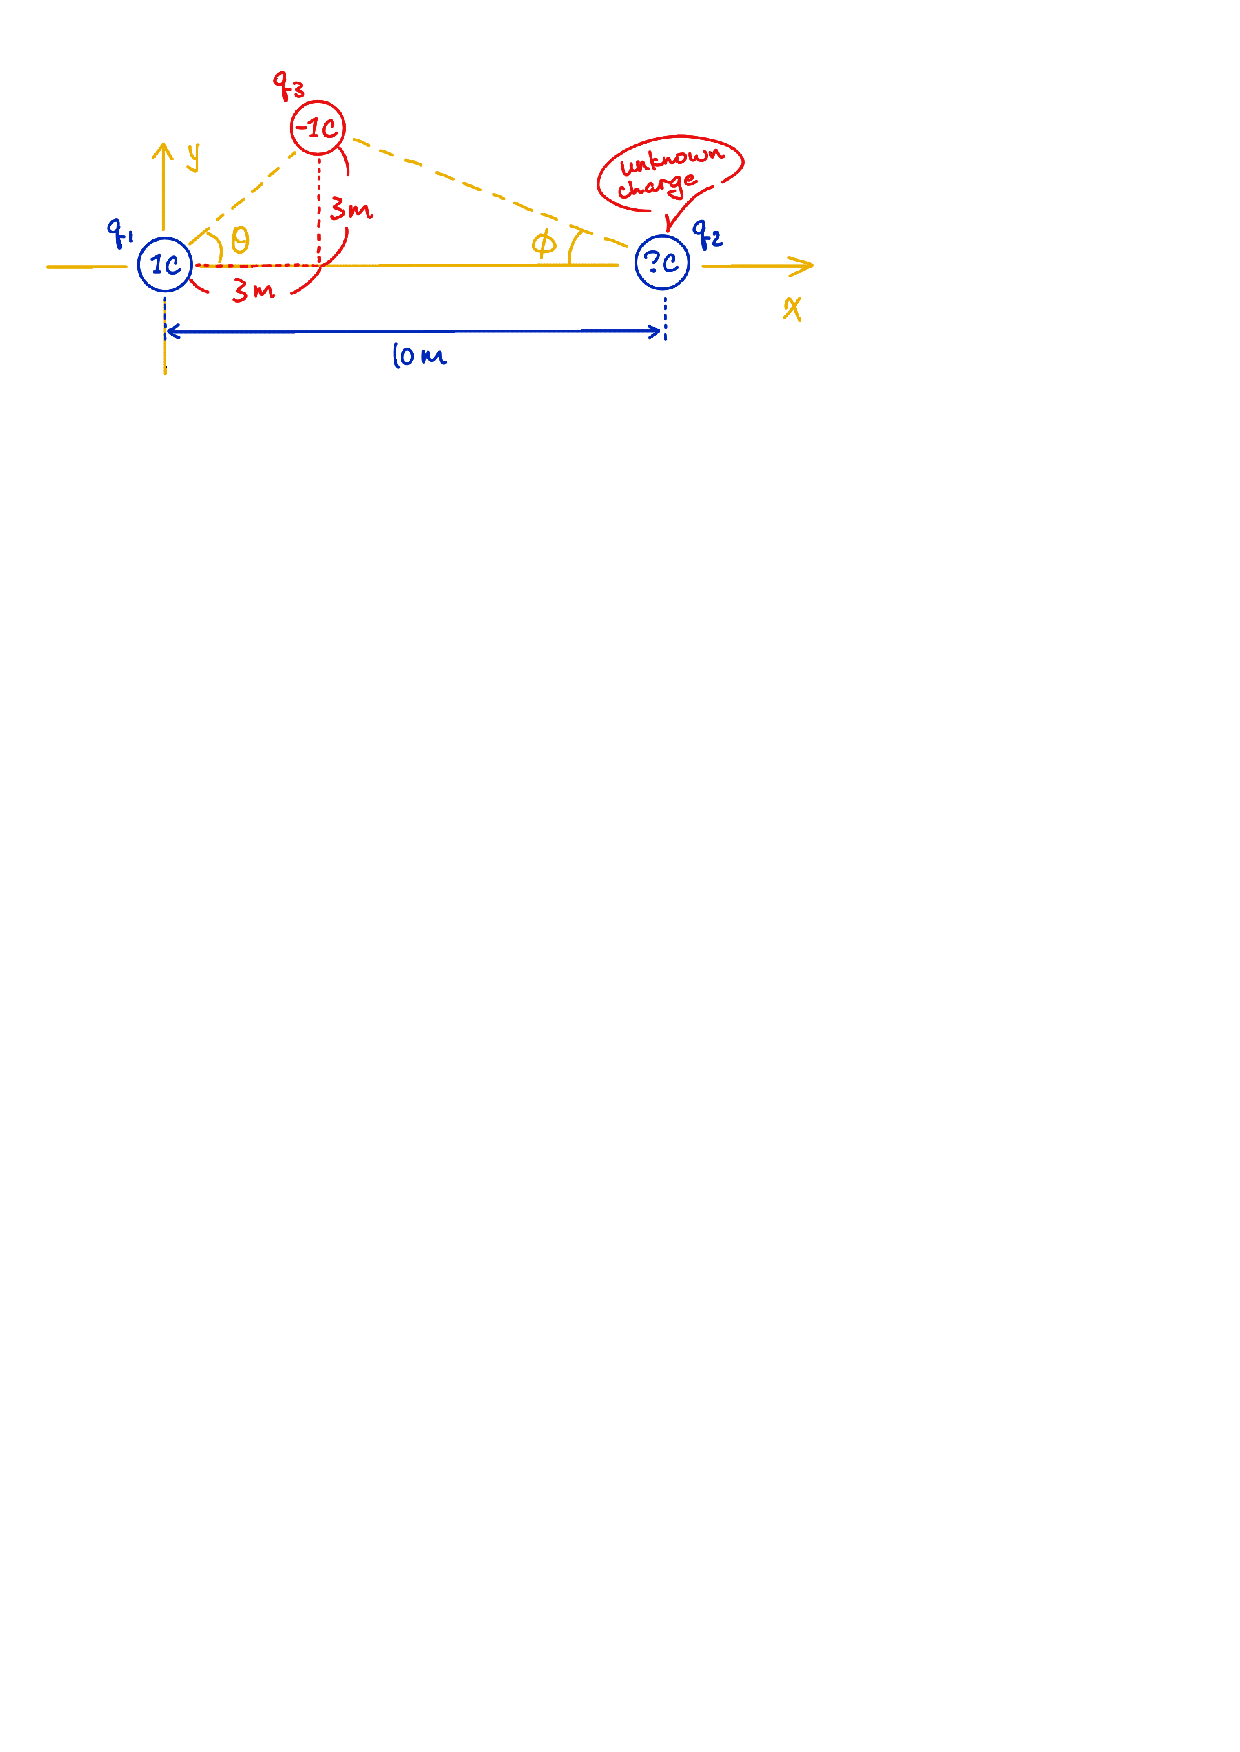
\includegraphics[scale=0.8]{chargeTriangle}
\end{center}
\noindent Now in this case, suppose we do not know the charge (or the sign) of $q_2$ fixed at $\vec{x}_2 = (10 ,0)$\,m, but we know that $q_1 = 1\,$C is fixed at $\vec{x}_1 = (0,0)$\,m and
$q_3=-1$\,C placed at $\vec{x}_3 = (3,3)$\,m has a tendency to move directly downwards (the electric force it experiences pulls it directly downwards). Find the electric field $\vec{E} = (E_x,E_y)$ at the position $\vec{x}_3 = (3,3)$\,m, due to the source charges $q_1$ and $q_2$. \footnote{Hint: $q_3$ wants to move directly downwards, that means the horizontal components of the forces acting on $q_3$ sum up to zero. There are only two electric forces acting on $q_3$, by the other two charges. Use some trigonometry to decompose the forces acting on $q_3$, then find the charge of $q_2$, and use that to find the electric field at $\vec{x}_3$ by superpositioning the electric fields due to $q_1$ and $q_2$.}


\newpage
\section*{Problem 1}
Field lines come out from positive charges and terminate at negative charges. Also note that $q_2 = 2$\,C is ``stronger" than $q_1 = 1$\,C.
\begin{center}
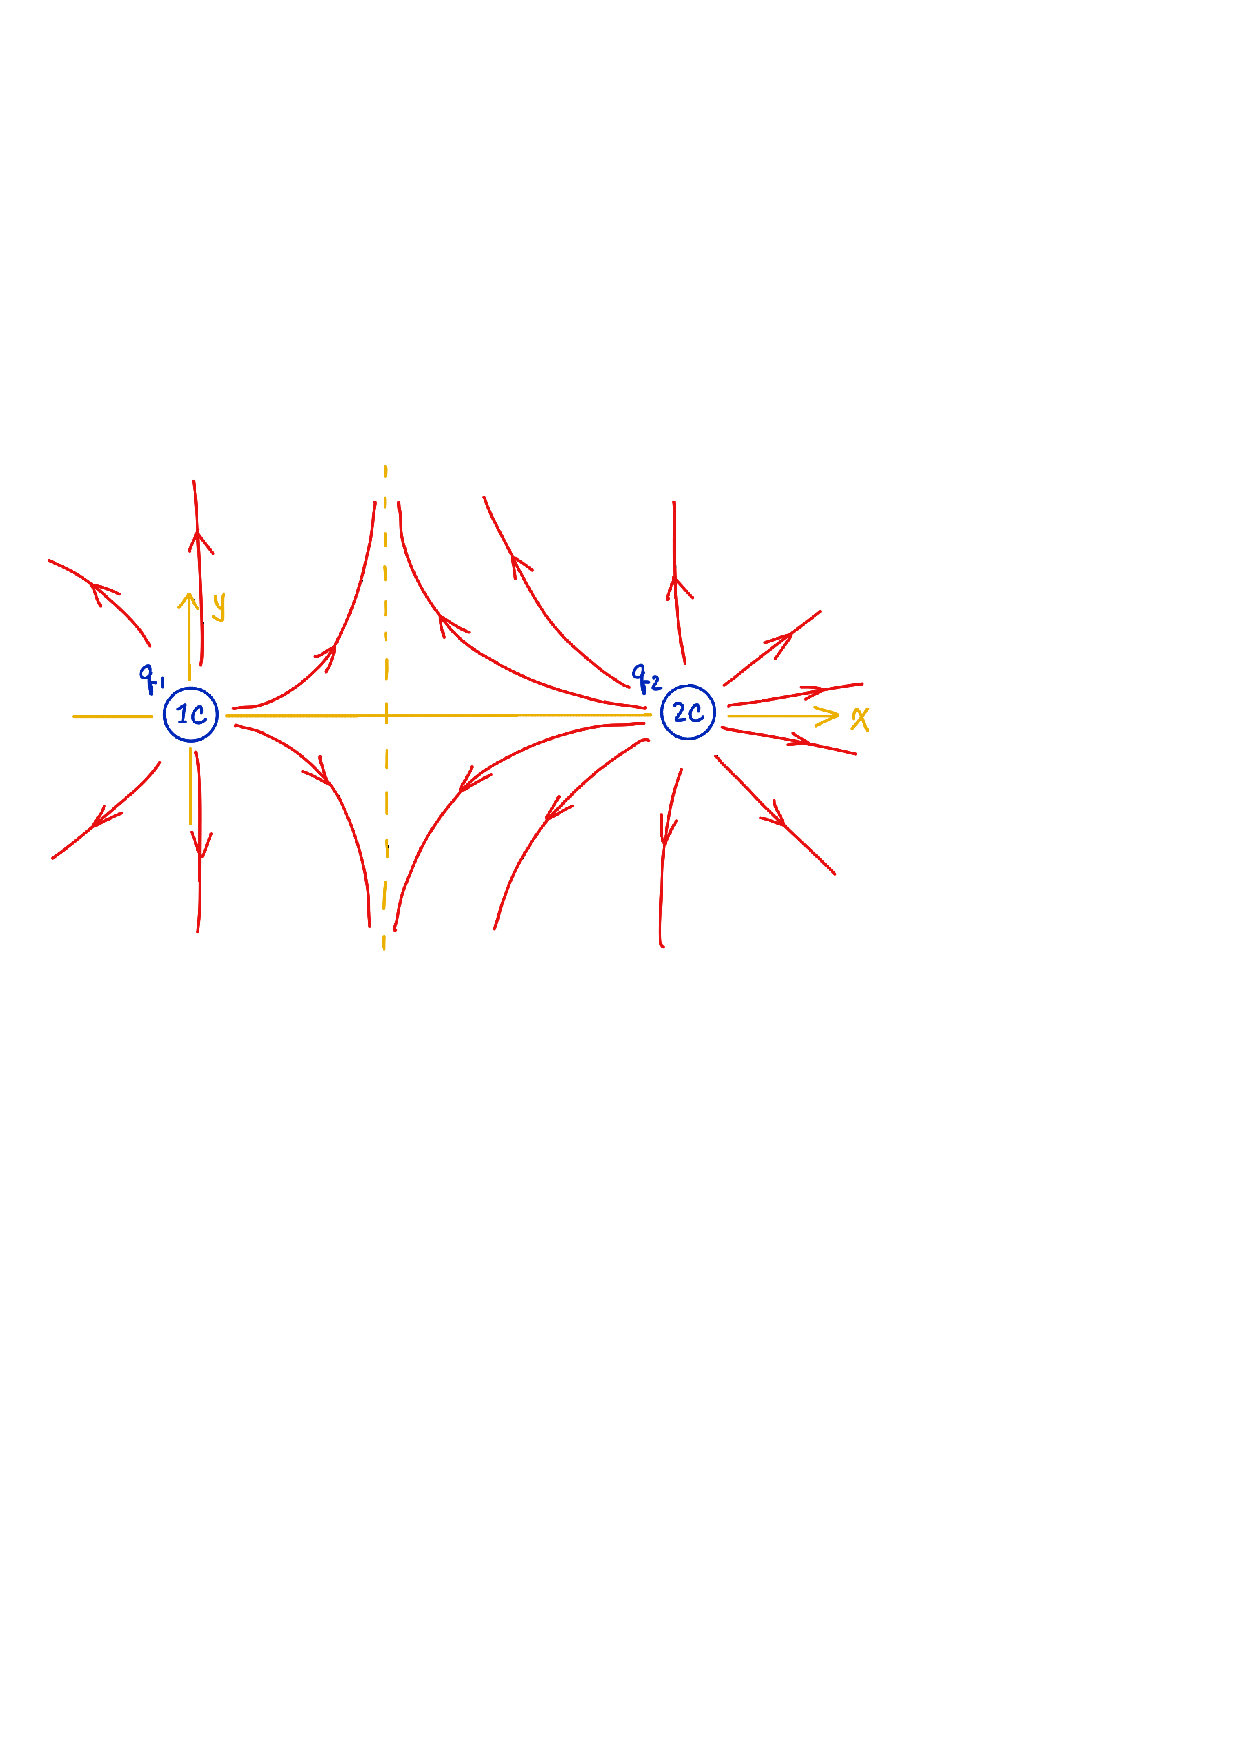
\includegraphics[scale=0.8]{field}
\end{center}
Here $q_3$ experiences two forces, one due to $q_1$ and the other one due to $q_2$. Since $q_3$ is negative, while $q_1$ and $q_2$ are positive, we deduce that both $q_1$ and $q_2$ are ``pulling" $q_3$. In particular, $q_1$ is dragging $q_3$ towards $q_1$ on the left, and $q_2$ is dragging $q_3$ towards $q_2$ on the right. Therefore, the location where $q_3$ experiences zero net force is the place where the two forces due to $q_1$ and $q_2$ cancel out exactly. It is not hard to see that this location must be somewhere between $q_1$ and $q_2$ on the horizontal $x$-axis. \\

To find such a location, let us suppose $q_3$ experiences zero net force when it is located at $(x,0)$ with $0< x< 10$ (because we want $q_3$ to be between $q_1$ and $q_2$). Then its distance to $q_1$ is $x$, and its distance to $q_2$ is $10-x$, so we can write the two forces
\begin{align*}
\vec{F}_{13} = -\frac{k|q_1 q_3|}{x^2}\hat{x}\,,\qquad
\vec{F}_{23} = \frac{k|q_2 q_3|}{(10-x)^2}\hat{x}\,.
\end{align*}
The first one is negative because $q_1$ is dragging $q_3$ to the left. Both forces have their $y$-components vanish because $q_1$ and $q_2$ want to drag $q_3$ directly towards them. The net force $q_3$ experiences is thus the sum
\begin{align*}
\vec{F}_{\text{net}} = \vec{F}_{13} + \vec{F}_{23} = kq_3 \left(\frac{|q_2|}{(10-x)^2} -\frac{|q_1|}{x^2}\right)\,\hat{x} \,.
\end{align*}
We want to find where $\vec{F}_{\text{net}} = (0,0)$, thus it suffices to find where
\begin{align*}
\frac{|q_2|}{(10-x)^2} - \frac{|q_1|}{x^2} = 0\,.
\end{align*}
Now we plug in the numbers, 
\begin{align*}
\frac{2}{(10-x)^2} - \frac{1}{x^2} = 0\,.
\end{align*}
There are many ways to solve for $x$, and here is one of them, 
\begin{align*}
\frac{2}{(10-x)^2} &= \frac{1}{x^2} \,,\\
2x^2 &= (10-x)^2\,,\\
2x^2 &= 100 - 20x + x^2 \,.
\end{align*}
We obtain a quadratic equation, using the quadratic formula we obtain 
\begin{align*}
x = 4.14\,\text{m}\,.
\end{align*}
There is another solution $x = -24.14$\,m, but that one is not physical.\\

Now we want to find the electric force acting on $q_2$, if we place $q_3$ at $\vec{x}_3 = (4.14,\,0)$\,m. In this case, since we want to find the force on $q_2$, the ``other" charges that are pulling or pushing $q_2$ are $q_1$ and $q_3$. Therefore, $q_2$ is treated as a test charge, experiencing forces by the source charges $q_1$ and $q_3$. Here $q_1$ and $q_2$ have the same sign, so they repel each other, and thus $q_2$ experiences a force to the right (positive sign) due to $q_1$, 
\begin{align*}
\vec{F}_{12} = \frac{k|q_1q_2|}{(\text{distance between }q_1 \text{ and }q_2\text{)}^2}\,\hat{x} =\left( \frac{8.99 \cdot 10^9\cdot 1 \cdot 2}{10^2}\,\text{N}\right)\,\hat{x} = \left(1.80 \cdot 10^8\,\text{N}\right)\, \hat{x}\,.
\end{align*}
On the other hand, $q_3$ and $q_2$ have opposite signs, thus $q_3$ is pulling $q_2$ to the left (negative sign for the force). Now we write
\begin{align*}
\vec{F}_{32} = -\frac{k|q_3q_2|}{(\text{distance between }q_3 \text{ and }q_2\text{)}^2}\,\hat{x} =\left( -\frac{8.99 \cdot 10^9\cdot |-1| \cdot 2}{(10-4.14)^2}\,\text{N}\right)\,\hat{x} = \left(-5.24 \cdot 10^8\,\text{N}\right)\, \hat{x}\,.
\end{align*} 
Adding these two forces together we get the net force experienced by $q_2$,
\begin{align*}
\vec{F}_{\text{net}} =\vec{F}_{12} + \vec{F}_{32} =\left(-3.44\cdot 10^{8}\,\text{N}\right) \hat{x}\,.
\end{align*}
After summing the effects due to both $q_1$ and $q_3$, we see that  $q_2$ is getting pulled to the left (hence the negative sign in the net force). This is because $q_2$ is closer to $q_3$ which pulls $q_2$ to the left. \\

In the problem, it is said that $q_3$ is initially at $\vec{x}_3 = (5,0)$, to the right of the point where it experiences zero net force. Therefore, $q_2$ (on the right) would have a stronger effect on $q_3$, trying to pull $q_3$ to the right. However, $q_3$ is initially moving to the left with $\vec{v}_i = (-1,0)$\,m/s, so $q_3$ will be moving to the left but slowing down. Depending on whether $q_3$ can pass through $x = 4.14$\,m (the point where the forces due $q_1$ and $q_2$ balance out), there will be two different end results: \\
\begin{enumerate}
\item $q_3$ is initially moving to the left, slowing down, able to pass through $x= 4.14$\,m. In this case it enters the region where the force due to the left charge $q_1$ dominates, which pulls $q_3$ towards $q_1$, so $q_3$ will end up hitting $q_1$.\\
\item $q_3$ is initially moving to the left, slowing down, but unable to pass through $x= 4.14$\,m. Then in this case, it will ``turn around" before reaching $x = 4.14$\,m, and remain in the region where the force due to the right charge $q_2$ dominates, which pulls $q_3$ towards $q_2$, so $q_3$ will end up hitting $q_2$.
\end{enumerate}


\section*{Problem 2}
In this configuration, we know that $q_3$ experiences a net force that has a zero $x$-component, because the net force is directly downwards. The force that $q_1$ exerts on $q_3$ has the form
\begin{align*}
\vec{F}_{13} = \left(
-\frac{k|q_1q_3|}{r^2}\, \cos(\theta)\,,\
-\frac{k|q_1q_3|}{r^2}\, \sin(\theta)
\right)\,,
\end{align*}
where $r = \sqrt{3^2 + 3^2}\,\text{m}= 3\sqrt{2}$\,m indicates the distance between charge $q_1$ and charge $q_3$. The $\sin$ and $\cos$ are there to extract the $x$- and $y$-components of $\vec{F}_{13}$. We are able to do this (extract the components) because the magnitude of $\vec{F}_{13}$ is $|kq_1q_3|/r^2$ based on Coulomb's law. Similarly, we write down
\begin{align*}
\vec{F}_{23} = \left(
\frac{k|q_2q_3|}{R^2}\, \cos(\phi)\,,\
-\frac{k|q_2q_3|}{R^2}\, \sin(\phi)
\right)
\end{align*}
where $R = \sqrt{(10-3)^2 + 3^2} = \sqrt{58}\,$m, and $\phi$ is the angle indicated on the original figure. The additional negative sign is added in the $y$-component to ensure that $\vec{F}_{23}$ is dragging $q_3$ towards $q_2$ (so we want the force to be pointing right-down, positive in $x$-component and negative in $y$-component). \\

Using the trigonometry here, we see that 
\begin{align*}
\sin(\theta) = \frac{3}{\sqrt{3^2 + 3^2}} = \frac{1}{\sqrt{2}}\,,\qquad
\cos(\theta) = \frac{3}{\sqrt{3^2 + 3^2}} = \frac{1}{\sqrt{2}}\,.
\end{align*}
\begin{align*}
\sin(\phi) = \frac{3}{\sqrt{(10-3)^2 + 3^2}} = \frac{3}{\sqrt{58}}\,,\qquad
\cos(\phi) = \frac{(10-3)}{\sqrt{(10-3)^2 + 3^2}} = \frac{7}{\sqrt{58}}\,.
\end{align*}
So we conclude 
\begin{align*}
\vec{F}_{13} = \left(
-\frac{k|q_1q_3|}{18}\,\frac{1}{\sqrt{2}} \,,\
-\frac{k|q_1q_3|}{18}\,\frac{1}{\sqrt{2}}
\right)\,,\qquad
\vec{F}_{23} = \left(
\frac{k|q_2q_3|}{58}\,\frac{7}{\sqrt{58}} \,,\
-\frac{k|q_2q_3|}{58}\,\frac{3}{\sqrt{58}} \,.
\right)\\
\end{align*}

The statement in the problem is that the sum of these two forces is directly downwards, that is the $x$-components should cancel each other, 
\begin{align*}
-\frac{k|q_1q_3|}{18}\,\frac{1}{\sqrt{2}} +
\frac{k|q_2q_3|}{58}\,\frac{7}{\sqrt{58}}= k|q_3|\left( -\frac{|q_1|}{18\sqrt{2}}+\frac{7|q_2|}{58\sqrt{58}}\right) = 0\,,
\end{align*}
from which we can find $q_2$ by plugging in the value of $q_1$, 
\begin{align*}
-\frac{1}{18\sqrt{2}}+\frac{7|q_2|}{58\sqrt{58}} = 0\,,
\end{align*}
thus $q_2 = 2.48$\,C (the sign of $q_2$ has to be positive, otherwise the $x$-components cannot cancel each other out based on the geometry, as both forces will be pushing $q_3$ to the left if $q_2$ was negative). Now the electric field at $\vec{x}_3 = (3,3)$\,m is in fact the electric force experienced by $q_3$ divided by $q_3$ (note that $q_3$ is negative), that is, 
\begin{align*}
\vec{E}(\vec{x}_3) = \frac{\vec{F}_{13} + \vec{F}_{23}}{q_3} = \left(
\frac{k|q_1|}{18\sqrt{2}} - \frac{k|q_2|}{58}\frac{7}{\sqrt{58}}\,,\
\frac{k|q_1|}{18\sqrt{2}} + \frac{k|q_2|}{58}\frac{3}{\sqrt{58}}
\right) \, \text{N/C}\,.
\end{align*}
Plug in $q_1 = 1$\,C and $q_2=2.48$\,C we find
\begin{align*}
\vec{E}(\vec{x}_3) = \left(0,\ 5.04\cdot 10^8\right)\,\text{N/C}\,.
\end{align*}
\newpage
\begin{center}

\includegraphics[scale=0.15]{wk2}\\
\hfill\break
A squirrel at the University of Michigan ... $\mathbb{GO\ BLUE}$\,!\\
\end{center}
\end{document}


